\chapter{Deep Sentiment}

Real-world information oftentimes come in several modalities. For instance, in speech recognition, humans integrate audio and visual information to understand speech, as was demonstrated by the McGurk effect \cite{mcgurk}. Separating what we see from what we hear seems like an easy task, but in the experiment conducted by McGurk, the subjects who were listening to a /{\em ba}/ sound with a visual /{\em ga}/ actually reported they were hearing a /{\em da}/. This is uncanny as even if you know the actual sound is a /{\em ba}/, you cannot stop your brain from interpreting it as a /{\em da}/.

Likewise, an image almost always come with a text as different interpretation can arise when a textual context is not provided, as shown in Figure \ref{ambiguous}:

\begin{figure}[H]
    \begin{subfigure}{.5\textwidth}
        \centering
        
\includegraphics[width=0.9\linewidth]{Images/scared.jpg}
        \caption{``Planes might just be the most frightening thing ever." \textbf{scared}}
    \end{subfigure}
    \begin{subfigure}{.5\textwidth}
        \centering
        
\includegraphics[width=0.9\linewidth]{Images/scared.jpg}
        \caption{``I hate it when people are taking too much space on planes." \textbf{angry}}
    \end{subfigure}
    \caption{Different meanings with different captions.}
    \label{ambiguous}
\end{figure}

Exploiting both visual and textual information is therefore key to understand the user's emotional state. Deep Sentiment is the name of the deep neural network incorporating visual recognition and text analysis.

%%%%%%%%%%%%%%%%%%%%%%%%%%%%%%%%%%%%%%%%%%%%%%%%%%%%%%%%%%%%
%%%%%%%%%%%%%%%%%%%%  NEW SECTION   %%%%%%%%%%%%%%%%%%%%%%%%
%%%%%%%%%%%%%%%%%%%%%%%%%%%%%%%%%%%%%%%%%%%%%%%%%%%%%%%%%%%%
\section{The Architecture}

Deep Sentiment builds on the models we have seen before as shown in Figure \ref{deep-sentiment}:

\begin{figure}[H]
    \centering
    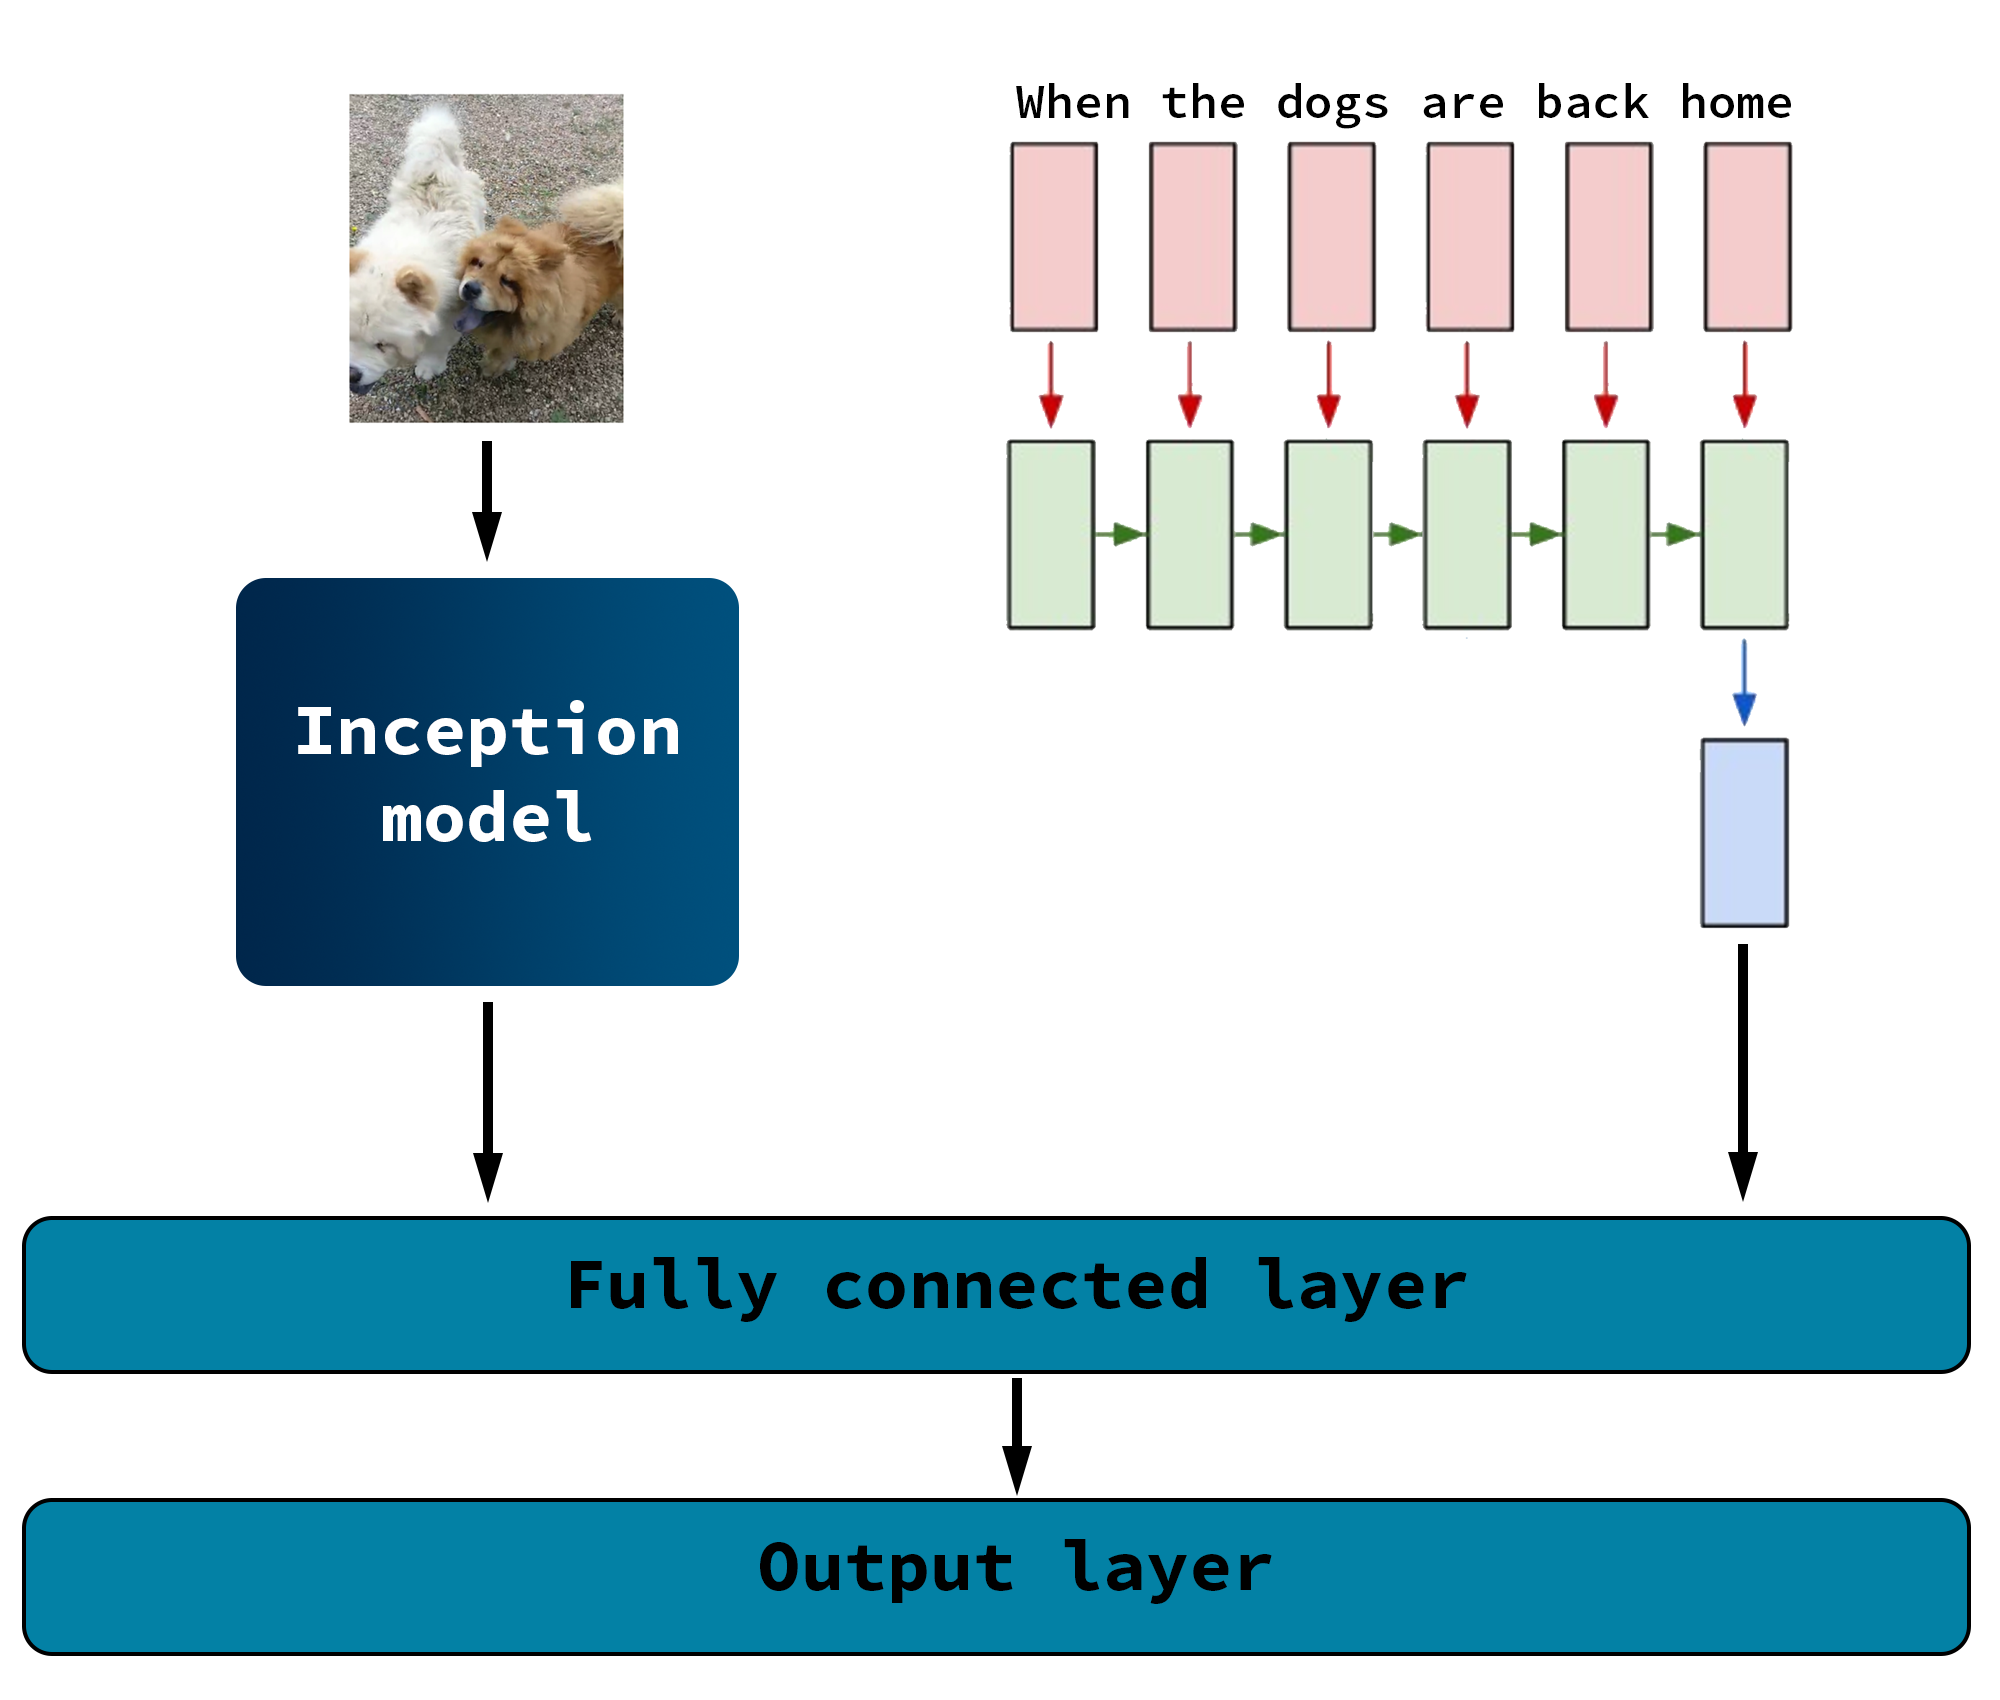
\includegraphics[width=\textwidth]{Images/deep-sentiment.png}
    \caption{Deep Sentiment architecture}
    \label{deep-sentiment}
\end{figure}

\begin{enumerate}
    \item The image go through the pre-trained Inception model that will extract features from the images, more precisely with 128 neurons in the last Inception 
    layer.
    \item The text is embedded in a high-dimensional space with Word2Vec and will be fed to an LSTM with a 2048 neurons output layer.
    \item The two outputs are concatenated to form the `Fully connected layer' in the graph with 2176 neurons. 
    \item The final layer with 6 neurons one for each basic emotion.
    \item A softmax layer to give the probability distribution of the emotional state of the user.
\end{enumerate}

\section{Results}
Deep Sentiment was trained with:
\begin{itemize}[topsep=0pt]
    \itemsep-1em
    \item 10,000 steps
    \item Mini-batch size of 32
    \item Adam optimizer with initial learning rate of $1\mathrm{e}{-3}$
    \item Learning rate decay of $\frac{1}{2}$ every 1000 steps
\end{itemize}

The training process of the Inception fine-tuning was monitored thanks to Tensorboard:
\begin{figure}[H]
    \centering
    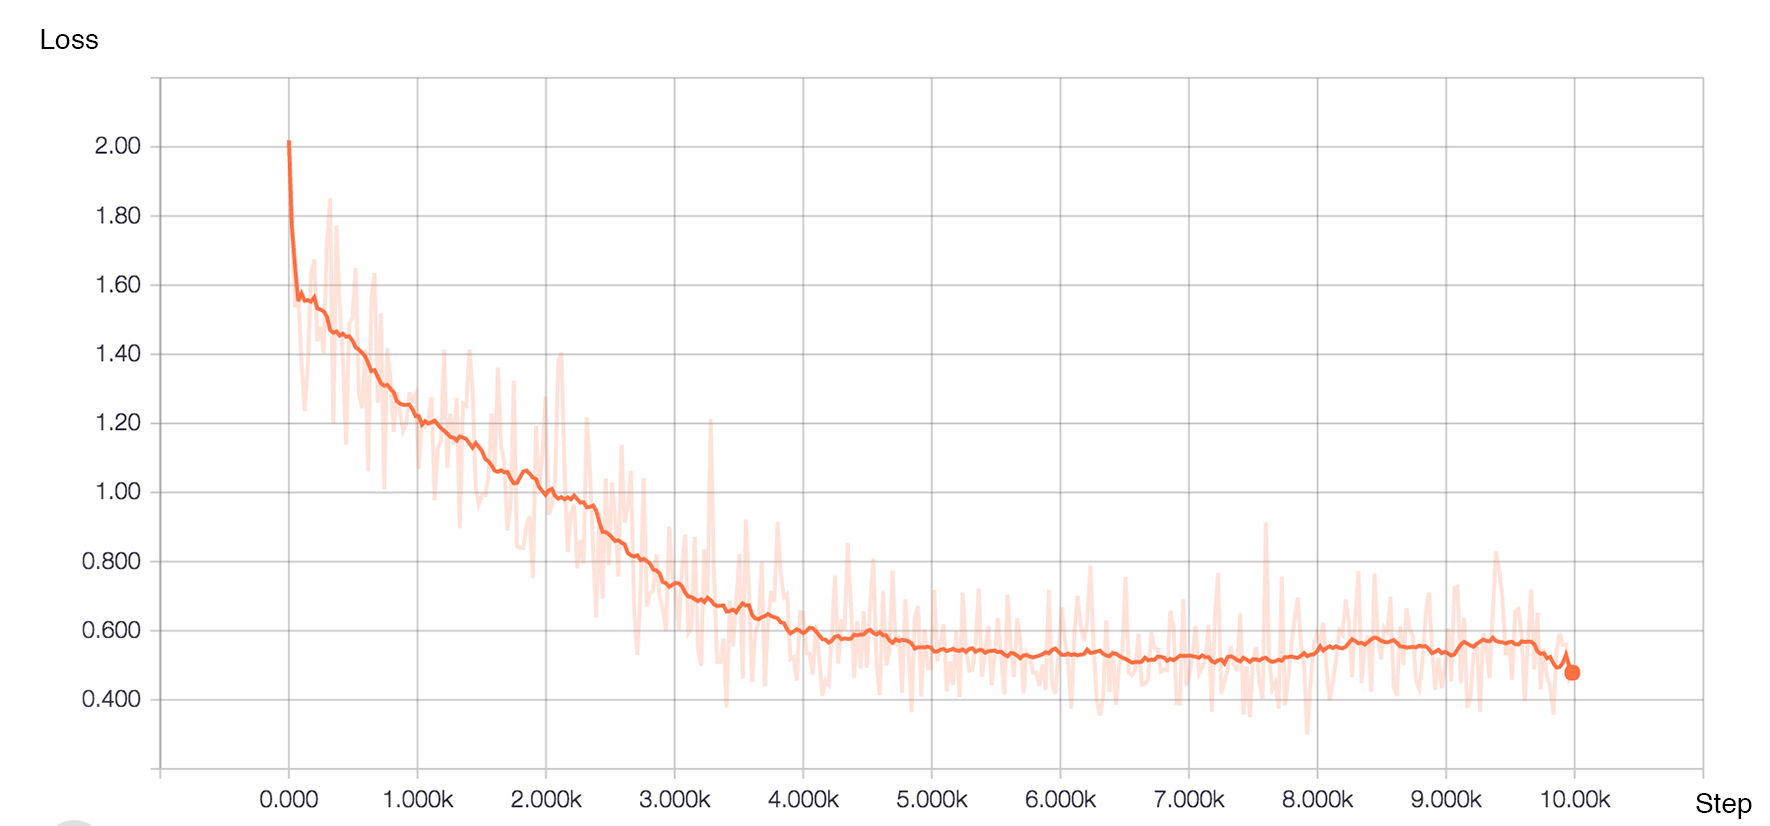
\includegraphics[width=\textwidth]{Images/image_text_model_loss_cleaned.jpg}
    \caption{Loss function of Deep Sentiment}
\end{figure}

\begin{figure}[H]
    \centering
    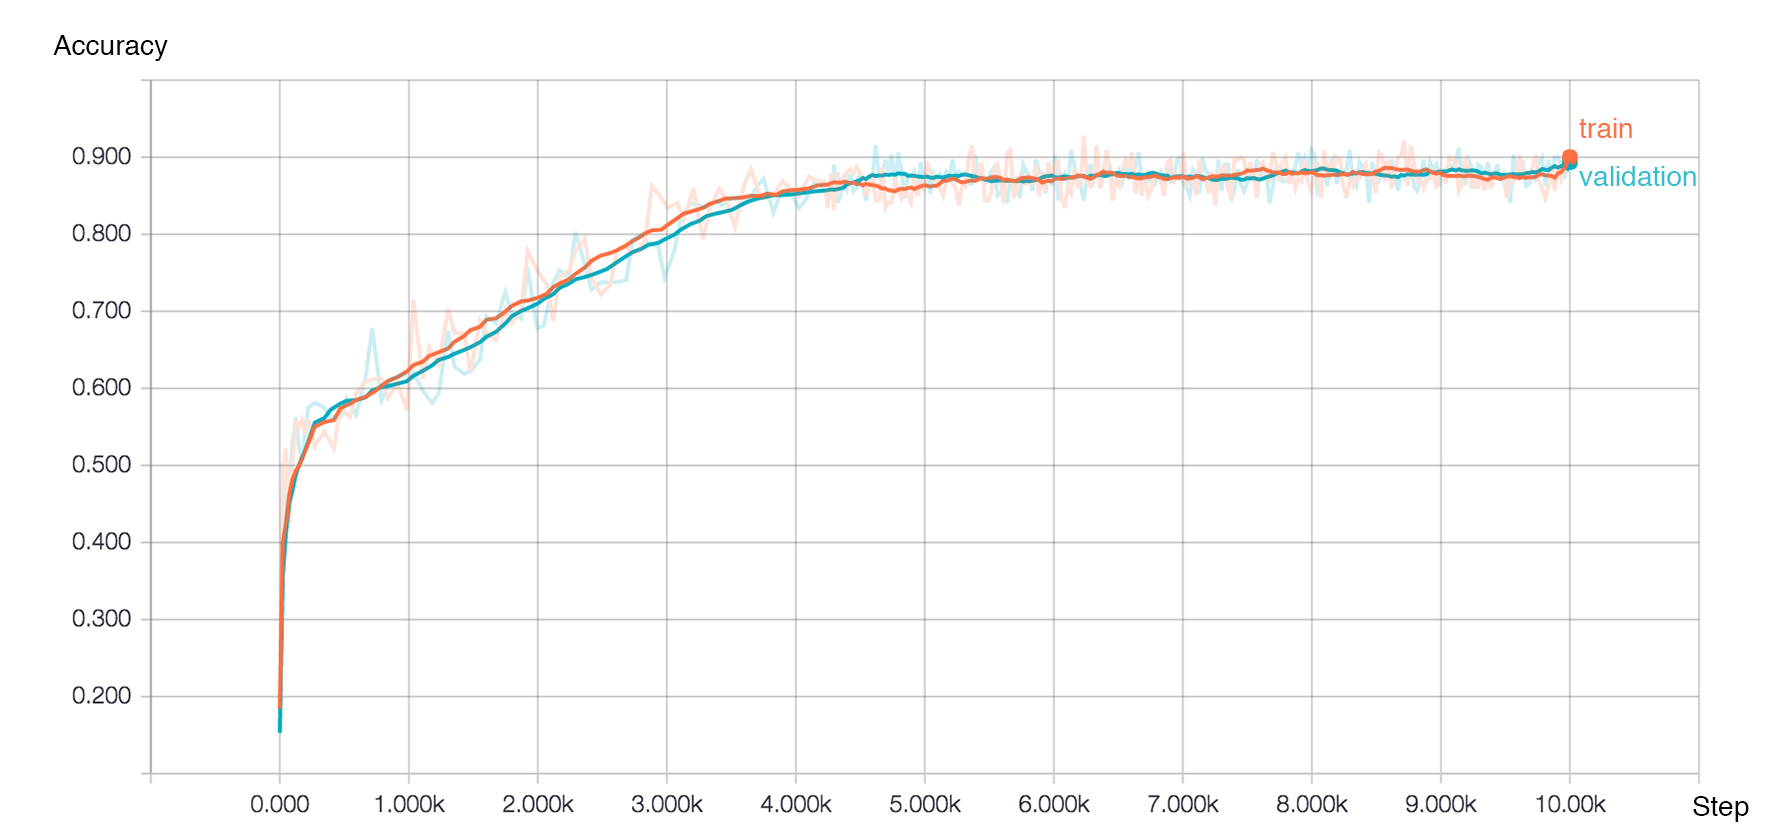
\includegraphics[width=\textwidth]{Images/image_text_model_accuracies_cleaned.jpg}
    \caption{Train/validation accuracies of Deep Sentiment}
\end{figure}

graph with the other models as well.

90\% train accuracy and 89\% test accuracy!

\newpage
\section{Emotion visualisation}
We can generate an image that maximises the score of a certain emotion by performing gradient ascent on a randomly initialised image \cite{class-vis}.

More concretely, let $I$ be an image and $y$ be a target emotion. Let us denote by $s_y(I)$ the score of class $y$ for the image $I$, that is one of the six neurons right before the softmax layer. We want to generate an image with a high score for emotion $y$ by solving the problem:
\begin{equation}
I^* = \text{arg\,max}_I ~s_y(I) - R(I)
\end{equation}

with $R(I)$ a regulariser that contains both explicit and implicit regularisation we will describe shortly.

Note that we're maximising the unnormalised class scores $s_y(I)$ and not the probabilities returned by the softmax: $\frac{s_y(I)}{\sum_c s_c(I)}$. The reason is that maximising the softmax probabilities can be achieved by minimising the scores of the other emotions. Instead, we want to make sure the optimisation concentrates on the emotion we want to visualise. 

\subsection{Regularisation}

The explicit regulariser is the $L_2$ decay: $R(I) = \lambda \Vert I \Vert_2^2$ that prevents extreme pixel values from dominating the generated image. Those pixel values do not occur naturally in real images and are not useful for visualisation.

The implicit regularisations are \cite{class-vis2}:
\begin{enumerate}
    \item \textbf{Gaussian blur:} Gradient ascent tends to produce image with high frequency information. What are frequencies in images? To put it simply, each image 
    is made of various frequencies: start with the average colour (low frequency) and slowly add higher frequencies wavelengths to build the details of the image.
    
    An image with high frequency information causes high activations but are not realistic nor interpretable as shown by Nguyen et al. \cite{nguyen}. High frequency 
    information are penalised using a Gaussian blur step on image $I: \text{GaussianBlur}(I, \theta_{\text{blur}})$ with $\theta_{\text{blur}}$ the standard deviation of the 
    Gaussian kernel used in the blur step. Blurring an image is computationally expensive and as such, we're only blurring every $\theta_{\text{blur-every}}$ steps.
    \item \textbf{Pixel clipping:} After performing $L_2$ decay and Gaussian blur, that suppress high amplitude and high frequency information, we're left with images 
    with pixel values that are small and smooth. However, each pixel will still be non-zero and contribute a little bit to the gradient. We want to discard the contribution of 
    unimportant pixels and focus only on the main object. That can be done by setting pixels with small norm (over the red, green, blue channels) to zero. The threshold  
    $\theta_{\text{small-norm}}$ for the norm is set to be a percentile of all pixel norms in the image.
\end{enumerate}

\subsection{Generated images}

We performed gradient ascent on a randomly initialised image using the following parameters:
\begin{itemize}
    \item $L_2$ regularisation parameter: $\lambda = 0.001$.
    \item In Gaussian blur, $\theta_{\text{blur}} = 0.5$ and $\theta_{\text{blur-every}} = 10$.
    \item In pixel clipping, $\theta_{\text{small-norm}}$ is the norm of the $10^{\text{th}}$ percentile.
    \item 500 gradient updates.
\end{itemize}

Maximising over the emotion `happy' yielded:

\begin{figure}[H]
    \centering
    
\includegraphics[width=0.6\textwidth]{Images/happy_gradient.png}
    \caption{Generated image maximising happiness}
\end{figure}

\newpage
\section{Generate text posts}

We can tweak Deep Sentiment to instead make the neural network generate text by feeding an image. The network will be trained to predict the next word of the text as shown in Figure \ref{deep-prediction}:

\begin{figure}[H]
    \centering
    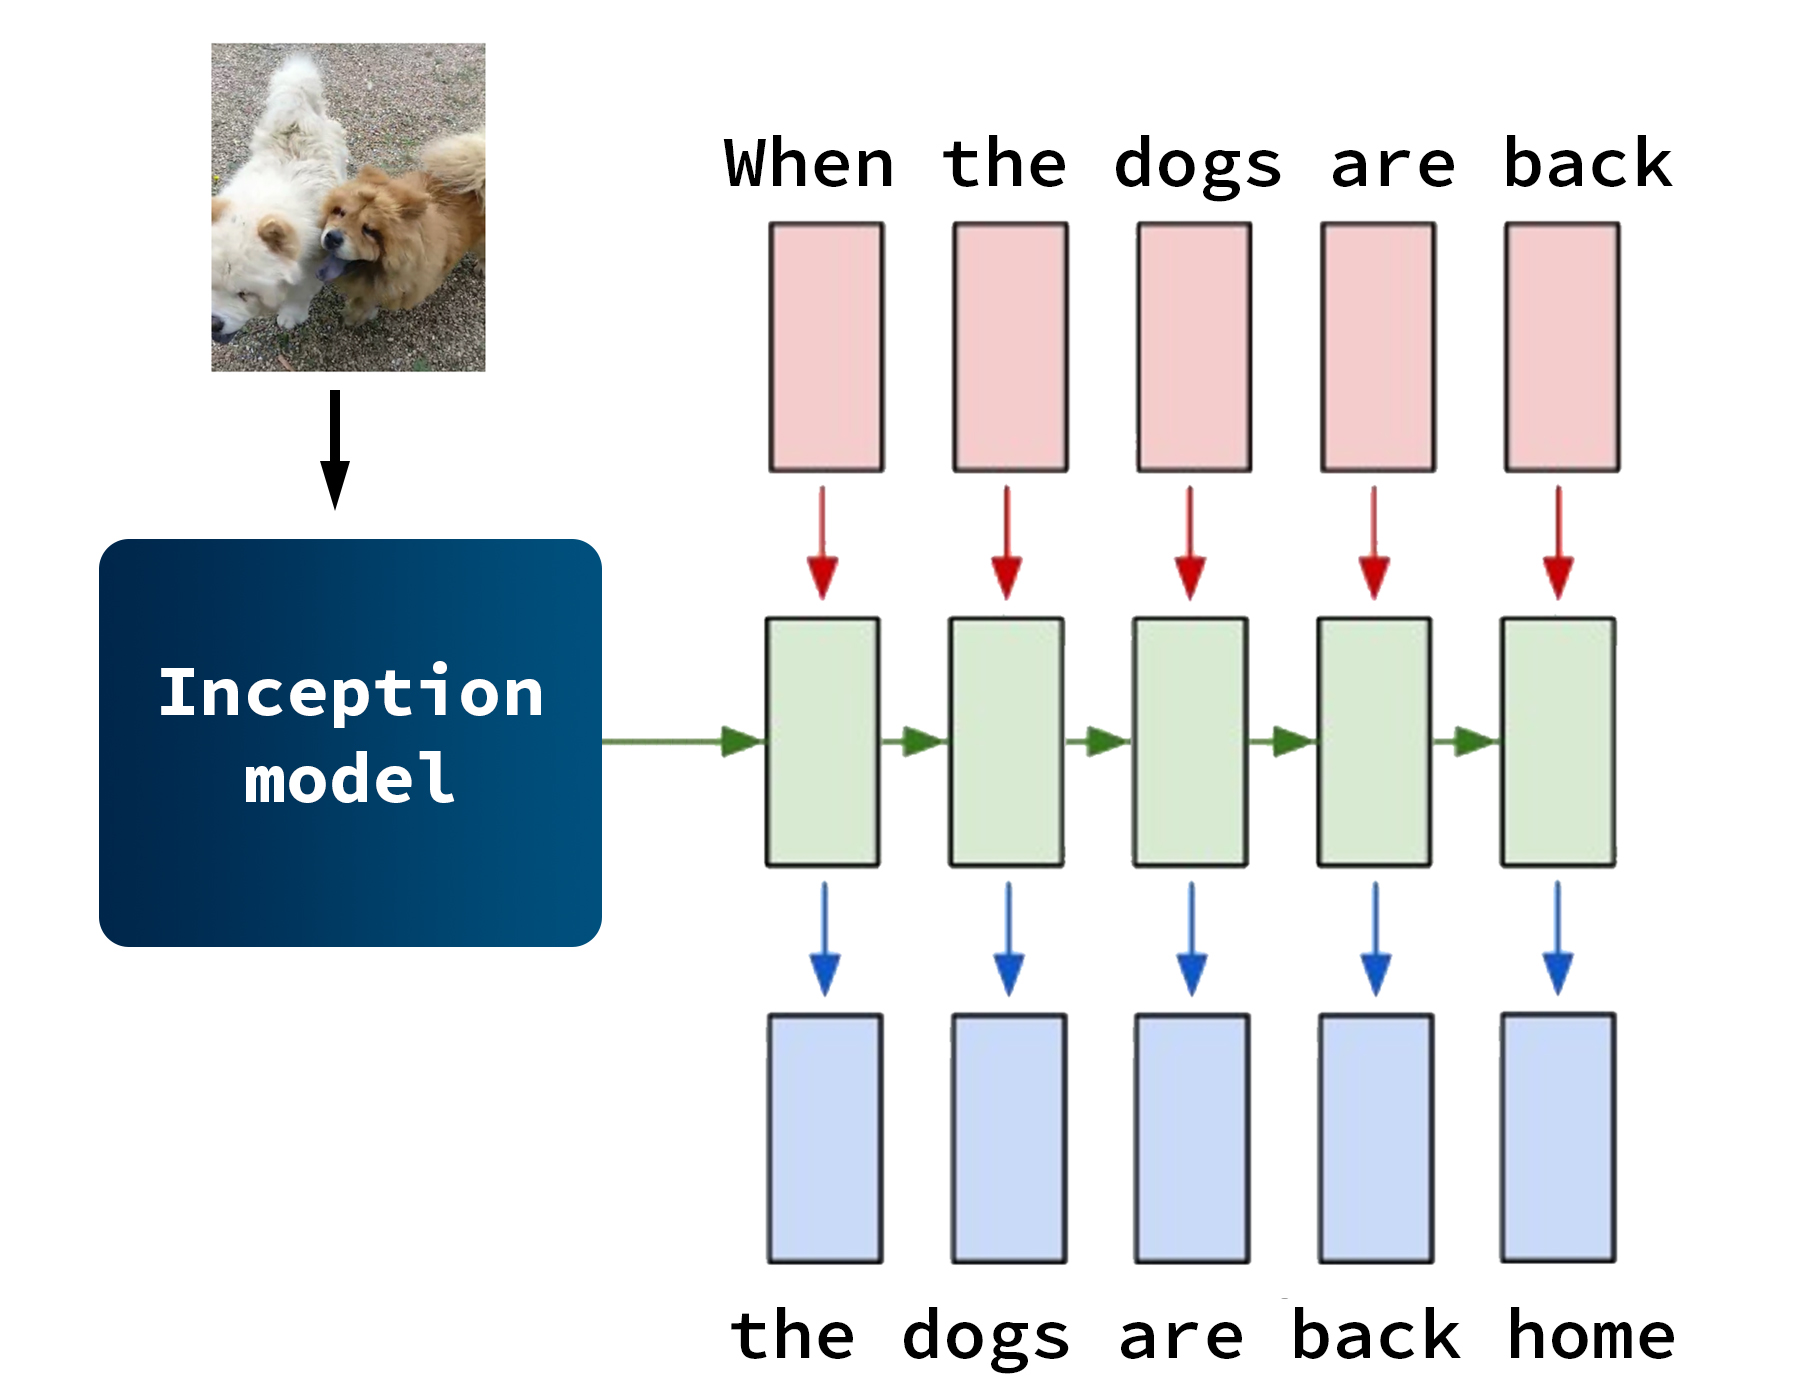
\includegraphics[width=\textwidth]{Images/deep-prediction.jpg}
    \caption{Deep Sentiment for text generation}
\end{figure}













